
\begin{table}[ht]
    \centering
    \caption{Point estimator performance, ordered by MSE (error = $0.5*\sigma$)}
    
\begin{tabular}{lrrrr}
\toprule
\multicolumn{1}{l}{Method} & \multicolumn{1}{c}{MSE} & \multicolumn{1}{c}{Bias} & \multicolumn{1}{c}{Variance} & \multicolumn{1}{c}{Average Runtime} \\
 & (000's years) & (years) & (000's years) & (seconds)\\
\midrule
BA-MLE & 244 & -22 & 244 & 0.00003\\
GRIWM-BA (q=0.5) & 245 & 95 & 236 & 13.88254\\
STRAUSS & 246 & -23 & 245 & 0.00002\\
SI-UGM & 251 & 117 & 237 & 2.33059\\
MINMI & 253 & 119 & 239 & 0.00047\\
\addlinespace
MLE & 428 & 455 & 221 & 0.00002\\
SI-RM & 428 & 455 & 221 & 0.06072\\
GRIWM (q=0.05) & 1276 & -993 & 291 & 2.35887\\
\bottomrule
\end{tabular}

    \label{tab:table-sim-exp-point-error0.5}
\end{table}

\begin{table}[ht]
    \centering
    \caption{Point estimator performance, ordered by MSE (error = $2*\sigma$)}
    
\begin{tabular}{lrrrr}
\toprule
\multicolumn{1}{l}{Method} & \multicolumn{1}{c}{MSE} & \multicolumn{1}{c}{Bias} & \multicolumn{1}{c}{Variance} & \multicolumn{1}{c}{Average Runtime} \\
 & (000's years) & (years) & (000's years) & (seconds)\\
\midrule
MINMI & 492 & 27 & 492 & 0.00071\\
SI-UGM & 502 & 65 & 498 & 1.68008\\
GRIWM-BA (q=0.5) & 505 & -278 & 428 & 13.94220\\
MLE & 507 & 254 & 443 & 0.00002\\
SI-RM & 507 & 254 & 443 & 0.05993\\
\addlinespace
BA-MLE & 543 & -234 & 489 & 0.00002\\
Strauss & 554 & -248 & 493 & 0.00002\\
GRIWM (q=0.05) & 2507 & -1408 & 526 & 2.36410\\
\bottomrule
\end{tabular}

    \label{tab:table-sim-exp-point-error2}
\end{table}

\begin{figure}[ht]
    \centering
    \includesvg[inkscapelatex=false, width=\linewidth]{figures/plot-sim-exp-point-est-grid.svg}
    \caption{Plots of different point estimate metrics from the simulation studies. Left to right, top to bottom: MSE, Bias, Variance, Average Runtime.}
    \label{fig:sim-exp-grid}
\end{figure}

\begin{table}[ht]
    \centering
    \caption{Confidence Interval Widths}
    
\begin{tabular}{lrrrr}
\toprule
\multicolumn{1}{c}{Method} & \multicolumn{4}{c}{Average Width} \\
 & 0*$\sigma$ & 0.5*$\sigma$ & 1*$\sigma$ & 2*$\sigma$\\
\midrule
SI-RM & 2054.55 & 2375.39 & 2500.86 & 2459.19\\
SI-UGM & 1961.14 & 2091.09 & 2964.30 & 2351.53\\
MINMI & 1917.16 & 2077.86 & 2932.73 & 2329.95\\
GRIWM-corrected & 0.00 & 548.08 & 1949.67 & 1047.99\\
GRIWM & 0.00 & 608.33 & 2163.50 & 1162.65\\
\bottomrule
\end{tabular}

    \label{tab:table-sim-exp-width}
\end{table}

\begin{table}[ht]
    \centering
    \caption{Confidence Interval Run Times against measurement error.}
    
\begin{tabular}{lrrrr}
\toprule
\multicolumn{1}{c}{Method} & \multicolumn{4}{c}{Average Runtime} \\
 & 0*$\sigma$ & 0.5*$\sigma$ & 1*$\sigma$ & 2*$\sigma$\\
\midrule
SI-RM & 0.0564 & 0.0607 & 0.0599 & 0.0599\\
SI-UGM & 4.7066 & 2.3306 & 1.6801 & 1.9374\\
MINMI & 0.0000 & 0.0013 & 0.0021 & 0.0014\\
GRIWM-BA (q=0.5) & 13.8988 & 13.8825 & 13.9422 & 13.9010\\
GRIWM (q=0.05) & 2.3355 & 2.3589 & 2.3641 & 18.1072\\
\bottomrule
\end{tabular}

    \label{tab:table-sim-exp-runtime}
\end{table}

% \begin{figure}[ht]
%     \centering
%     \includesvg[inkscapelatex=false, width=\linewidth]{figures/applications-hists.svg}
%     \caption{Histograms of the four megafauna species' datasets. From left to right: the cave bear, cave hyena, Eurasian woolly mammoth, and steppe bison.}
%     \label{fig:applications-histograms}
% \end{figure}

\begin{figure}[ht]
    \centering
    % Created by tikzDevice version 0.12.3.1 on 2022-11-18 13:23:06
% !TEX encoding = UTF-8 Unicode
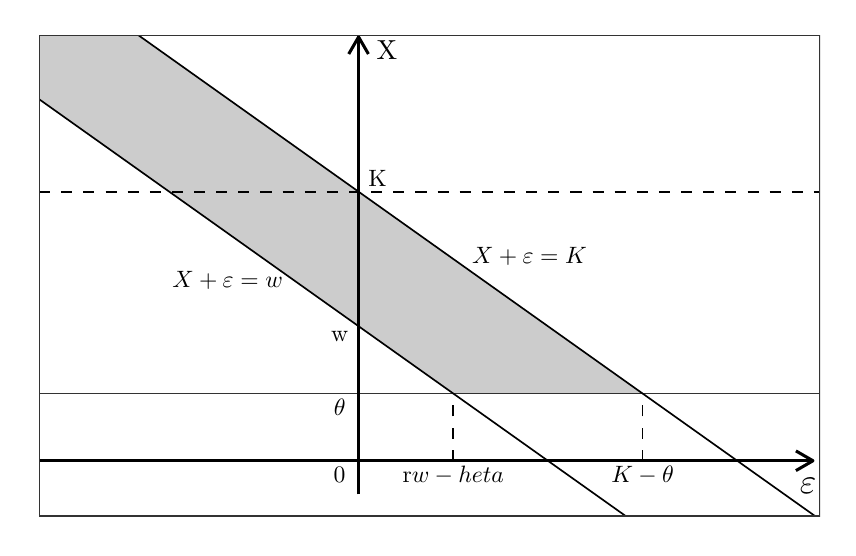
\begin{tikzpicture}[node distance = 2cm, auto, scale=0.5, transform shape, x=1pt,y=1pt]
\definecolor{fillColor}{RGB}{255,255,255}
\path[use as bounding box,fill=fillColor,fill opacity=0.00] (0,0) rectangle (578.16,361.35);
\begin{scope}
\path[clip] (  0.00,  0.00) rectangle (578.16,361.35);
\definecolor{drawColor}{RGB}{255,255,255}
\definecolor{fillColor}{RGB}{255,255,255}

\path[draw=drawColor,line width= 0.6pt,line join=round,line cap=round,fill=fillColor] (  0.00,  0.00) rectangle (578.16,361.35);
\end{scope}
\begin{scope}
\path[clip] (  8.25,  8.25) rectangle (572.66,355.85);
\definecolor{fillColor}{RGB}{255,255,255}

\path[fill=fillColor] (  8.25,  8.25) rectangle (572.66,355.85);
\definecolor{drawColor}{RGB}{0,0,0}

\path[draw=drawColor,line width= 1.1pt,line join=round] (-444.99, 48.36) -- (567.53, 48.36);

\path[draw=drawColor,line width= 1.1pt,line join=round] (555.21, 41.24) --
	(567.53, 48.36) --
	(555.21, 55.47);

\path[draw=drawColor,line width= 1.1pt,line join=round] (239.14, 24.05) -- (239.14,354.63);

\path[draw=drawColor,line width= 1.1pt,line join=round] (246.26,342.31) --
	(239.14,354.63) --
	(232.03,342.31);

\node[text=drawColor,anchor=base,inner sep=0pt, outer sep=0pt, scale=  1.99] at (259.67,338.05) {X};

\node[text=drawColor,anchor=base,inner sep=0pt, outer sep=0pt, scale=  2.56] at (564.11, 24.95) {$\varepsilon$};

\path[draw=drawColor,line width= 0.6pt,line join=round] (-556.16,807.97) -- (1137.07,-395.26);

\path[draw=drawColor,line width= 0.6pt,line join=round] (-556.16,710.74) -- (1137.07,-492.49);
\definecolor{fillColor}{RGB}{0,0,0}

\path[fill=fillColor,fill opacity=0.20] (-444.99,728.97) --
	(-438.15,724.11) --
	(-431.31,719.25) --
	(-424.46,714.39) --
	(-417.62,709.53) --
	(-410.78,704.67) --
	(-403.94,699.80) --
	(-397.10,694.94) --
	(-390.26,690.08) --
	(-383.42,685.22) --
	(-376.57,680.36) --
	(-369.73,675.50) --
	(-362.89,670.63) --
	(-356.05,665.77) --
	(-349.21,660.91) --
	(-342.37,656.05) --
	(-335.53,651.19) --
	(-328.69,646.33) --
	(-321.84,641.47) --
	(-315.00,636.60) --
	(-308.16,631.74) --
	(-301.32,626.88) --
	(-294.48,622.02) --
	(-287.64,617.16) --
	(-280.80,612.30) --
	(-273.95,607.43) --
	(-267.11,602.57) --
	(-260.27,597.71) --
	(-253.43,592.85) --
	(-246.59,587.99) --
	(-239.75,583.13) --
	(-232.91,578.27) --
	(-226.07,573.40) --
	(-219.22,568.54) --
	(-212.38,563.68) --
	(-205.54,558.82) --
	(-198.70,553.96) --
	(-191.86,549.10) --
	(-185.02,544.23) --
	(-178.18,539.37) --
	(-171.33,534.51) --
	(-164.49,529.65) --
	(-157.65,524.79) --
	(-150.81,519.93) --
	(-143.97,515.07) --
	(-137.13,510.20) --
	(-130.29,505.34) --
	(-123.45,500.48) --
	(-116.60,495.62) --
	(-109.76,490.76) --
	(-102.92,485.90) --
	(-96.08,481.03) --
	(-89.24,476.17) --
	(-82.40,471.31) --
	(-75.56,466.45) --
	(-68.71,461.59) --
	(-61.87,456.73) --
	(-55.03,451.87) --
	(-48.19,447.00) --
	(-41.35,442.14) --
	(-34.51,437.28) --
	(-27.67,432.42) --
	(-20.83,427.56) --
	(-13.98,422.70) --
	( -7.14,417.83) --
	( -0.30,412.97) --
	(  6.54,408.11) --
	( 13.38,403.25) --
	( 20.22,398.39) --
	( 27.06,393.53) --
	( 33.90,388.67) --
	( 40.75,383.80) --
	( 47.59,378.94) --
	( 54.43,374.08) --
	( 61.27,369.22) --
	( 68.11,364.36) --
	( 74.95,359.50) --
	( 81.79,354.63) --
	( 88.64,349.77) --
	( 95.48,344.91) --
	(102.32,340.05) --
	(109.16,335.19) --
	(116.00,330.33) --
	(122.84,325.47) --
	(129.68,320.60) --
	(136.52,315.74) --
	(143.37,310.88) --
	(150.21,306.02) --
	(157.05,301.16) --
	(163.89,296.30) --
	(170.73,291.43) --
	(177.57,286.57) --
	(184.41,281.71) --
	(191.26,276.85) --
	(198.10,271.99) --
	(204.94,267.13) --
	(211.78,262.27) --
	(218.62,257.40) --
	(225.46,252.54) --
	(232.30,247.68) --
	(239.14,242.82) --
	(245.99,237.96) --
	(252.83,233.10) --
	(259.67,228.23) --
	(266.51,223.37) --
	(273.35,218.51) --
	(280.19,213.65) --
	(287.03,208.79) --
	(293.88,203.93) --
	(300.72,199.07) --
	(307.56,194.20) --
	(314.40,189.34) --
	(321.24,184.48) --
	(328.08,179.62) --
	(334.92,174.76) --
	(341.76,169.90) --
	(348.61,165.03) --
	(355.45,160.17) --
	(362.29,155.31) --
	(369.13,150.45) --
	(375.97,145.59) --
	(382.81,140.73) --
	(389.65,135.87) --
	(396.50,131.00) --
	(403.34,126.14) --
	(410.18,121.28) --
	(417.02,116.42) --
	(423.86,111.56) --
	(430.70,106.70) --
	(437.54,101.83) --
	(444.38, 96.97) --
	(444.38, 96.97) --
	(437.54, 96.97) --
	(430.70, 96.97) --
	(423.86, 96.97) --
	(417.02, 96.97) --
	(410.18, 96.97) --
	(403.34, 96.97) --
	(396.50, 96.97) --
	(389.65, 96.97) --
	(382.81, 96.97) --
	(375.97, 96.97) --
	(369.13, 96.97) --
	(362.29, 96.97) --
	(355.45, 96.97) --
	(348.61, 96.97) --
	(341.76, 96.97) --
	(334.92, 96.97) --
	(328.08, 96.97) --
	(321.24, 96.97) --
	(314.40, 96.97) --
	(307.56, 96.97) --
	(300.72,101.83) --
	(293.88,106.70) --
	(287.03,111.56) --
	(280.19,116.42) --
	(273.35,121.28) --
	(266.51,126.14) --
	(259.67,131.00) --
	(252.83,135.87) --
	(245.99,140.73) --
	(239.14,145.59) --
	(232.30,150.45) --
	(225.46,155.31) --
	(218.62,160.17) --
	(211.78,165.03) --
	(204.94,169.90) --
	(198.10,174.76) --
	(191.26,179.62) --
	(184.41,184.48) --
	(177.57,189.34) --
	(170.73,194.20) --
	(163.89,199.07) --
	(157.05,203.93) --
	(150.21,208.79) --
	(143.37,213.65) --
	(136.52,218.51) --
	(129.68,223.37) --
	(122.84,228.23) --
	(116.00,233.10) --
	(109.16,237.96) --
	(102.32,242.82) --
	( 95.48,247.68) --
	( 88.64,252.54) --
	( 81.79,257.40) --
	( 74.95,262.27) --
	( 68.11,267.13) --
	( 61.27,271.99) --
	( 54.43,276.85) --
	( 47.59,281.71) --
	( 40.75,286.57) --
	( 33.90,291.43) --
	( 27.06,296.30) --
	( 20.22,301.16) --
	( 13.38,306.02) --
	(  6.54,310.88) --
	( -0.30,315.74) --
	( -7.14,320.60) --
	(-13.98,325.47) --
	(-20.83,330.33) --
	(-27.67,335.19) --
	(-34.51,340.05) --
	(-41.35,344.91) --
	(-48.19,349.77) --
	(-55.03,354.63) --
	(-61.87,359.50) --
	(-68.71,364.36) --
	(-75.56,369.22) --
	(-82.40,374.08) --
	(-89.24,378.94) --
	(-96.08,383.80) --
	(-102.92,388.67) --
	(-109.76,393.53) --
	(-116.60,398.39) --
	(-123.45,403.25) --
	(-130.29,408.11) --
	(-137.13,412.97) --
	(-143.97,417.83) --
	(-150.81,422.70) --
	(-157.65,427.56) --
	(-164.49,432.42) --
	(-171.33,437.28) --
	(-178.18,442.14) --
	(-185.02,447.00) --
	(-191.86,451.87) --
	(-198.70,456.73) --
	(-205.54,461.59) --
	(-212.38,466.45) --
	(-219.22,471.31) --
	(-226.07,476.17) --
	(-232.91,481.03) --
	(-239.75,485.90) --
	(-246.59,490.76) --
	(-253.43,495.62) --
	(-260.27,500.48) --
	(-267.11,505.34) --
	(-273.95,510.20) --
	(-280.80,515.07) --
	(-287.64,519.93) --
	(-294.48,524.79) --
	(-301.32,529.65) --
	(-308.16,534.51) --
	(-315.00,539.37) --
	(-321.84,544.23) --
	(-328.69,549.10) --
	(-335.53,553.96) --
	(-342.37,558.82) --
	(-349.21,563.68) --
	(-356.05,568.54) --
	(-362.89,573.40) --
	(-369.73,578.27) --
	(-376.57,583.13) --
	(-383.42,587.99) --
	(-390.26,592.85) --
	(-397.10,597.71) --
	(-403.94,602.57) --
	(-410.78,607.43) --
	(-417.62,612.30) --
	(-424.46,617.16) --
	(-431.31,622.02) --
	(-438.15,626.88) --
	(-444.99,631.74) --
	cycle;

\path[] (-444.99,728.97) --
	(-438.15,724.11) --
	(-431.31,719.25) --
	(-424.46,714.39) --
	(-417.62,709.53) --
	(-410.78,704.67) --
	(-403.94,699.80) --
	(-397.10,694.94) --
	(-390.26,690.08) --
	(-383.42,685.22) --
	(-376.57,680.36) --
	(-369.73,675.50) --
	(-362.89,670.63) --
	(-356.05,665.77) --
	(-349.21,660.91) --
	(-342.37,656.05) --
	(-335.53,651.19) --
	(-328.69,646.33) --
	(-321.84,641.47) --
	(-315.00,636.60) --
	(-308.16,631.74) --
	(-301.32,626.88) --
	(-294.48,622.02) --
	(-287.64,617.16) --
	(-280.80,612.30) --
	(-273.95,607.43) --
	(-267.11,602.57) --
	(-260.27,597.71) --
	(-253.43,592.85) --
	(-246.59,587.99) --
	(-239.75,583.13) --
	(-232.91,578.27) --
	(-226.07,573.40) --
	(-219.22,568.54) --
	(-212.38,563.68) --
	(-205.54,558.82) --
	(-198.70,553.96) --
	(-191.86,549.10) --
	(-185.02,544.23) --
	(-178.18,539.37) --
	(-171.33,534.51) --
	(-164.49,529.65) --
	(-157.65,524.79) --
	(-150.81,519.93) --
	(-143.97,515.07) --
	(-137.13,510.20) --
	(-130.29,505.34) --
	(-123.45,500.48) --
	(-116.60,495.62) --
	(-109.76,490.76) --
	(-102.92,485.90) --
	(-96.08,481.03) --
	(-89.24,476.17) --
	(-82.40,471.31) --
	(-75.56,466.45) --
	(-68.71,461.59) --
	(-61.87,456.73) --
	(-55.03,451.87) --
	(-48.19,447.00) --
	(-41.35,442.14) --
	(-34.51,437.28) --
	(-27.67,432.42) --
	(-20.83,427.56) --
	(-13.98,422.70) --
	( -7.14,417.83) --
	( -0.30,412.97) --
	(  6.54,408.11) --
	( 13.38,403.25) --
	( 20.22,398.39) --
	( 27.06,393.53) --
	( 33.90,388.67) --
	( 40.75,383.80) --
	( 47.59,378.94) --
	( 54.43,374.08) --
	( 61.27,369.22) --
	( 68.11,364.36) --
	( 74.95,359.50) --
	( 81.79,354.63) --
	( 88.64,349.77) --
	( 95.48,344.91) --
	(102.32,340.05) --
	(109.16,335.19) --
	(116.00,330.33) --
	(122.84,325.47) --
	(129.68,320.60) --
	(136.52,315.74) --
	(143.37,310.88) --
	(150.21,306.02) --
	(157.05,301.16) --
	(163.89,296.30) --
	(170.73,291.43) --
	(177.57,286.57) --
	(184.41,281.71) --
	(191.26,276.85) --
	(198.10,271.99) --
	(204.94,267.13) --
	(211.78,262.27) --
	(218.62,257.40) --
	(225.46,252.54) --
	(232.30,247.68) --
	(239.14,242.82) --
	(245.99,237.96) --
	(252.83,233.10) --
	(259.67,228.23) --
	(266.51,223.37) --
	(273.35,218.51) --
	(280.19,213.65) --
	(287.03,208.79) --
	(293.88,203.93) --
	(300.72,199.07) --
	(307.56,194.20) --
	(314.40,189.34) --
	(321.24,184.48) --
	(328.08,179.62) --
	(334.92,174.76) --
	(341.76,169.90) --
	(348.61,165.03) --
	(355.45,160.17) --
	(362.29,155.31) --
	(369.13,150.45) --
	(375.97,145.59) --
	(382.81,140.73) --
	(389.65,135.87) --
	(396.50,131.00) --
	(403.34,126.14) --
	(410.18,121.28) --
	(417.02,116.42) --
	(423.86,111.56) --
	(430.70,106.70) --
	(437.54,101.83) --
	(444.38, 96.97);

\path[] (444.38, 96.97) --
	(437.54, 96.97) --
	(430.70, 96.97) --
	(423.86, 96.97) --
	(417.02, 96.97) --
	(410.18, 96.97) --
	(403.34, 96.97) --
	(396.50, 96.97) --
	(389.65, 96.97) --
	(382.81, 96.97) --
	(375.97, 96.97) --
	(369.13, 96.97) --
	(362.29, 96.97) --
	(355.45, 96.97) --
	(348.61, 96.97) --
	(341.76, 96.97) --
	(334.92, 96.97) --
	(328.08, 96.97) --
	(321.24, 96.97) --
	(314.40, 96.97) --
	(307.56, 96.97) --
	(300.72,101.83) --
	(293.88,106.70) --
	(287.03,111.56) --
	(280.19,116.42) --
	(273.35,121.28) --
	(266.51,126.14) --
	(259.67,131.00) --
	(252.83,135.87) --
	(245.99,140.73) --
	(239.14,145.59) --
	(232.30,150.45) --
	(225.46,155.31) --
	(218.62,160.17) --
	(211.78,165.03) --
	(204.94,169.90) --
	(198.10,174.76) --
	(191.26,179.62) --
	(184.41,184.48) --
	(177.57,189.34) --
	(170.73,194.20) --
	(163.89,199.07) --
	(157.05,203.93) --
	(150.21,208.79) --
	(143.37,213.65) --
	(136.52,218.51) --
	(129.68,223.37) --
	(122.84,228.23) --
	(116.00,233.10) --
	(109.16,237.96) --
	(102.32,242.82) --
	( 95.48,247.68) --
	( 88.64,252.54) --
	( 81.79,257.40) --
	( 74.95,262.27) --
	( 68.11,267.13) --
	( 61.27,271.99) --
	( 54.43,276.85) --
	( 47.59,281.71) --
	( 40.75,286.57) --
	( 33.90,291.43) --
	( 27.06,296.30) --
	( 20.22,301.16) --
	( 13.38,306.02) --
	(  6.54,310.88) --
	( -0.30,315.74) --
	( -7.14,320.60) --
	(-13.98,325.47) --
	(-20.83,330.33) --
	(-27.67,335.19) --
	(-34.51,340.05) --
	(-41.35,344.91) --
	(-48.19,349.77) --
	(-55.03,354.63) --
	(-61.87,359.50) --
	(-68.71,364.36) --
	(-75.56,369.22) --
	(-82.40,374.08) --
	(-89.24,378.94) --
	(-96.08,383.80) --
	(-102.92,388.67) --
	(-109.76,393.53) --
	(-116.60,398.39) --
	(-123.45,403.25) --
	(-130.29,408.11) --
	(-137.13,412.97) --
	(-143.97,417.83) --
	(-150.81,422.70) --
	(-157.65,427.56) --
	(-164.49,432.42) --
	(-171.33,437.28) --
	(-178.18,442.14) --
	(-185.02,447.00) --
	(-191.86,451.87) --
	(-198.70,456.73) --
	(-205.54,461.59) --
	(-212.38,466.45) --
	(-219.22,471.31) --
	(-226.07,476.17) --
	(-232.91,481.03) --
	(-239.75,485.90) --
	(-246.59,490.76) --
	(-253.43,495.62) --
	(-260.27,500.48) --
	(-267.11,505.34) --
	(-273.95,510.20) --
	(-280.80,515.07) --
	(-287.64,519.93) --
	(-294.48,524.79) --
	(-301.32,529.65) --
	(-308.16,534.51) --
	(-315.00,539.37) --
	(-321.84,544.23) --
	(-328.69,549.10) --
	(-335.53,553.96) --
	(-342.37,558.82) --
	(-349.21,563.68) --
	(-356.05,568.54) --
	(-362.89,573.40) --
	(-369.73,578.27) --
	(-376.57,583.13) --
	(-383.42,587.99) --
	(-390.26,592.85) --
	(-397.10,597.71) --
	(-403.94,602.57) --
	(-410.78,607.43) --
	(-417.62,612.30) --
	(-424.46,617.16) --
	(-431.31,622.02) --
	(-438.15,626.88) --
	(-444.99,631.74);
\definecolor{drawColor}{RGB}{0,0,0}

\path[draw=drawColor,draw opacity=0.80,line width= 0.6pt,line join=round] (  8.25, 96.97) -- (572.66, 96.97);
\definecolor{drawColor}{RGB}{0,0,0}

\path[draw=drawColor,line width= 0.6pt,dash pattern=on 4pt off 4pt ,line join=round] (  8.25,242.82) -- (572.66,242.82);

\path[draw=drawColor,line width= 0.6pt,dash pattern=on 4pt off 4pt ,line join=round] (307.56, 48.36) -- (307.56, 96.97);

\path[draw=drawColor,line width= 0.6pt,dash pattern=on 4pt off 4pt ,line join=round] (444.38, 48.36) -- (444.38, 96.97);

\node[text=drawColor,anchor=base,inner sep=0pt, outer sep=0pt, scale=  1.71] at (252.83,246.66) {K};

\node[text=drawColor,anchor=base,inner sep=0pt, outer sep=0pt, scale=  1.71] at (225.46, 81.37) {$\theta$};

\node[text=drawColor,anchor=base,inner sep=0pt, outer sep=0pt, scale=  1.71] at (225.46,134.85) {w};

\node[text=drawColor,anchor=base,inner sep=0pt, outer sep=0pt, scale=  1.71] at (225.46, 32.76) {0};

\node[text=drawColor,anchor=base,inner sep=0pt, outer sep=0pt, scale=  1.71] at (307.56, 32.76) {r{$w-	heta$}};

\node[text=drawColor,anchor=base,inner sep=0pt, outer sep=0pt, scale=  1.71] at (444.38, 32.76) {$K-\theta$};

\node[text=drawColor,anchor=base west,inner sep=0pt, outer sep=0pt, scale=  1.71] at (321.24,190.76) {$X + \varepsilon = K$};

\node[text=drawColor,anchor=base east,inner sep=0pt, outer sep=0pt, scale=  1.71] at (184.41,173.74) {$X + \varepsilon = w$};
\definecolor{drawColor}{gray}{0.20}

\path[draw=drawColor,line width= 0.6pt,line join=round,line cap=round] (  8.25,  8.25) rectangle (572.66,355.85);
\end{scope}
\end{tikzpicture}

    \caption{Caption}
    \label{fig:my_label}
\end{figure}